% main.tex
% IEEE/ICE-style (IEEEtran conference) skeleton paper with TikZ figures.
% Intended as a handoff template: an undergrad can replace TODO blocks with data, plots, and results.

\documentclass[conference]{IEEEtran}

\IEEEoverridecommandlockouts

\usepackage{cite}
\usepackage{amsmath,amssymb,amsfonts}
\usepackage{graphicx}
\usepackage{booktabs}
\usepackage{multirow}
\usepackage{siunitx}
\usepackage{xcolor}
\usepackage[hidelinks]{hyperref}

\usepackage{algorithm}
\usepackage{algpseudocode}

\usepackage{tikz}
\usetikzlibrary{arrows.meta,positioning,shapes.geometric,calc,fit,backgrounds}

% ---------- Template helper macros ----------
\newcommand{\TODO}[1]{\textcolor{red}{\textbf{TODO:} #1}}
\newcommand{\OurSystem}{\textsc{OrinFlow}}

\newcommand{\etal}{\textit{et al.}}

% ---------- TikZ styles (IEEE/ICE-friendly small font) ----------
\tikzset{
  every node/.style={font=\footnotesize},
  block/.style={draw, rectangle, rounded corners, align=center, inner sep=3pt, minimum height=1.4em},
  smallblock/.style={draw, rectangle, rounded corners, align=center, inner sep=2pt, minimum height=1.1em},
  io/.style={draw, trapezium, trapezium left angle=70, trapezium right angle=110, align=center, inner sep=3pt},
  decision/.style={draw, diamond, aspect=2, align=center, inner sep=1pt},
  arrow/.style={-Latex, thick},
  dashedbox/.style={draw, dashed, rounded corners, inner sep=4pt}
}

\title{Real-Time IMU-Aided Camera-Based Surface Current Measurement on Edge Compute}

\author{
\IEEEauthorblockN{Devon Goshorn\IEEEauthorrefmark{1}, Douglas Cahl\IEEEauthorrefmark{2}, Yi Wang\IEEEauthorrefmark{2}}
\IEEEauthorblockA{\IEEEauthorrefmark{1}Department of Computer Engineering, University of South Carolina, Columbia, USA\\
email: devong@email.sc.edu}
\IEEEauthorblockA{\IEEEauthorrefmark{2}Department of Mechanical Engineering, University of South Carolina, Columbia, USA\\
email: douglesc@email.sc.edu, ywang@sc.edu}
}

\begin{document}
\maketitle

\begin{abstract}
Camera-based surface velocimetry enables non-contact measurement of water-surface currents for rivers, nearshore zones, and engineered channels. Prior work demonstrates accurate surface velocity estimation from video using large-scale PIV and variants (e.g., LSPIV/SSIV), space-time image velocimetry (STIV), and dense optical flow methods (including wavelet-based optical flow for nearshore foam tracking). However, end-to-end real-time performance on embedded platforms remains underreported, especially under platform motion where camera shake and pose drift contaminate apparent surface motion.
This paper defines, implements, and evaluates an IMU-aided real-time pipeline for estimating surface current fields on a Jetson Orin device. The system fuses synchronized camera and IMU streams for stabilization, planar rectification, and fast motion estimation, producing georeferenced velocity vectors with quantified latency, accuracy, and robustness. The manuscript is written as a reproducible system paper: it reports an error budget that links calibration, IMU integration, and motion estimation uncertainty to final velocity error, and it provides an experimental protocol for validation against in situ references.
\end{abstract}

\begin{IEEEkeywords}
surface current, image velocimetry, optical flow, STIV, embedded vision, IMU fusion, Jetson Orin, real time
\end{IEEEkeywords}

% ==========================================================
\section{Introduction}
Surface currents are central to hydrologic monitoring, flood response, sediment transport studies, and coastal safety. Conventional in situ sensors can be hazardous to deploy during extreme events, can disturb the flow, and often lack spatial coverage. Camera-based methods estimate surface velocities remotely by tracking advected texture, tracers, foam, or wave patterns, and can operate from fixed installations, bridges, UAVs, or mobile robots.

The systems-level question motivating this work is not whether video can measure flow, but whether it can do so \emph{reliably in real time on edge hardware} while the camera is moving. Platform motion induces optical flow unrelated to water motion, and the resulting bias becomes significant at shallow viewing angles and long ranges. Embedded deployment also introduces strict constraints on throughput, latency, power, and thermal stability.

This paper contributes a complete experimental-ready template for an IMU-aided embedded pipeline. The objective is to produce a manuscript that an  researcher can complete by collecting real data, running the experiments specified in Section~\ref{sec:experiments}, and populating the placeholders in Section~\ref{sec:results}.

% ==========================================================
\section{Related Work and Literature Review}
Camera-based surface velocimetry spans multiple domains. River and channel monitoring often uses correlation-based methods derived from particle image velocimetry, while nearshore and ocean applications frequently leverage foam tracking and/or wave dispersion. This section summarizes the foundations and highlights where embedded real-time, IMU-aided implementations remain an open engineering contribution.

\subsection{Large-Scale PIV and Cross-Correlation Methods}
Large-scale particle image velocimetry (LSPIV) adapts laboratory PIV to field-scale free surfaces by correlating interrogation windows between frames to estimate displacement. Muste \etal{} provide a widely cited field-oriented treatment of LSPIV for riverine environments, discussing practical considerations such as seeding, illumination, and orthorectification \cite{Muste2008LSPIV}.
Operational systems frequently incorporate robust pre-processing and site-specific calibration. Peña-Haro \etal{} describe an operational real-time monitoring system (DischargeKeeper) using surface-structure image velocimetry (SSIV), orthorectification, and robust filtering, emphasizing long-term continuous deployment and the practicalities of calibration and power management \cite{PenaHaro2021DischargeKeeper}.

\subsection{Space-Time Image Velocimetry (STIV) and Extensions}
STIV estimates streamwise velocity by constructing a space-time image along a chosen line and measuring the dominant stripe orientation, typically producing an average velocity over a time window. Fujita, Watanabe, and Tsubaki introduced STIV as an efficient non-intrusive monitoring method \cite{Fujita2007STIV}. Recent work expands STIV toward 2D flow fields and UAV settings. Han \etal{} propose 2D STIV for mountain rivers using UAV video, rotating candidate search lines to infer flow direction automatically \cite{Han2021TwoDSTIV}.

\subsection{Nearshore Surface Currents from Video and Optical Flow}
Nearshore currents can be estimated by tracking foam patterns in the surf zone. Dérian and Almar introduce ``Typhoon'', a wavelet-based dense optical flow method designed to retrieve instant surface currents from shore-based and UAV videos \cite{Derian2017Typhoon}. This line of work highlights the utility of dense optical flow for 2D current fields in environments with strong texture from foam.

\subsection{UAV Wave-Based Approaches}
Wave-based inversion methods estimate currents by analyzing the Doppler shift of the surface-wave dispersion relation in video-derived spectra. Streßer, Carrasco, and Horstmann demonstrate video-based estimation of surface currents using a low-cost quadcopter and spectral analysis, with open tooling associated with CopterCurrents \cite{Stresser2017CopterCurrents}.

\subsection{Embedded Real-Time Optical Flow}
While classical optical flow is computationally expensive, modern approaches improve efficiency via hardware acceleration or specialized neural architectures. NeuFlow reports real-time optical flow on edge devices including Jetson-class hardware, suggesting a viable option for embedded deployments when paired with careful systems engineering \cite{Zhang2024NeuFlow}.

\subsection{Synthesis and Gap Statement}
The literature establishes (i) accurate camera-only surface velocity estimation for rivers and coasts, (ii) operational continuous monitoring architectures for fixed installations, and (iii) efficient optical flow models for embedded inference. A gap remains in \emph{IMU-aided, end-to-end real-time} measurement of surface currents on embedded hardware under platform motion, with complete reporting of latency, uncertainty propagation, and field validation.

\begin{table}[t]
\caption{Representative camera-based surface flow measurement approaches and their relevance to embedded real-time IMU-aided systems.}
\label{tab:litreview}
\centering
\begin{tabular}{p{1.2cm}p{2.55cm}p{1.55cm}p{1.1cm}}
\toprule
Domain & Core method & Typical output & Example \\
\midrule
Rivers & LSPIV / SSIV (cross-correlation) & 2D surface velocity field or profile & \cite{Muste2008LSPIV,PenaHaro2021DischargeKeeper} \\
Rivers & STIV / 2D STIV (space-time stripes) & 1D or 2D average velocities & \cite{Fujita2007STIV,Han2021TwoDSTIV} \\
Nearshore & Dense optical flow on foam patterns & 2D current field & \cite{Derian2017Typhoon} \\
UAV/coast & Wave dispersion inversion & 2D current field & \cite{Stresser2017CopterCurrents} \\
Embedded & Efficient optical flow inference & Dense flow field (pixels/frame) & \cite{Zhang2024NeuFlow} \\
\bottomrule
\end{tabular}
\end{table}

% ==========================================================
\section{Problem Definition and System Requirements}
\label{sec:problem}
Let $I_t(\mathbf{p})$ denote an image at time $t$ with pixel location $\mathbf{p}=[u,v]^T$. The system outputs a georeferenced surface velocity field
\begin{equation}
\mathbf{u}(\mathbf{x},t) = [u_x(\mathbf{x},t),u_y(\mathbf{x},t)]^T,
\end{equation}
defined on water-surface coordinates $\mathbf{x}=[X,Y]^T$ in meters. Real-time operation is defined by a measured end-to-end latency $\tau$ from exposure midpoint to published velocity field, and a sustained throughput $f$ in frames per second (FPS), both measured on the target embedded device.

Platform motion is measured by an IMU providing angular velocity $\boldsymbol{\omega}(t)$ and linear acceleration $\mathbf{a}(t)$. The system assumes either a locally planar water surface or a piecewise planar approximation within the measurement region, sufficient for homography-based rectification.

\begin{table}[t]
\caption{Engineering requirements to be confirmed experimentally. Replace values with measured targets appropriate to the platform and mission.}
\label{tab:reqs}
\centering
\begin{tabular}{p{2.2cm}p{1.25cm}p{2.9cm}}
\toprule
Requirement & Target & Operational interpretation \\
\midrule
Latency $\tau$ & \TODO{e.g., $<\SI{200}{ms}$} & From exposure midpoint to published vector field \\
Throughput $f$ & \TODO{e.g., $\ge \SI{15}{FPS}$} & Sustained over \TODO{N} minutes without thermal throttling \\
Velocity error & \TODO{e.g., $<\SI{0.1}{m/s}$} & Compared to reference sensor in Section~\ref{sec:experiments} \\
Robustness & \TODO{quantify} & Performance across lighting, glare, low texture, and motion \\
Power & \TODO{e.g., $\le \SI{15}{W}$} & Average draw during continuous operation \\
\bottomrule
\end{tabular}
\end{table}

% ==========================================================
\section{System Overview}
\label{sec:system}
The hardware stack consists of a monocular camera, a 6-axis or 9-axis IMU, and an NVIDIA Jetson Orin module. The software stack implements synchronization, stabilization, rectification, motion estimation, post-processing, and publication of velocities.

\begin{figure}[t]
\centering
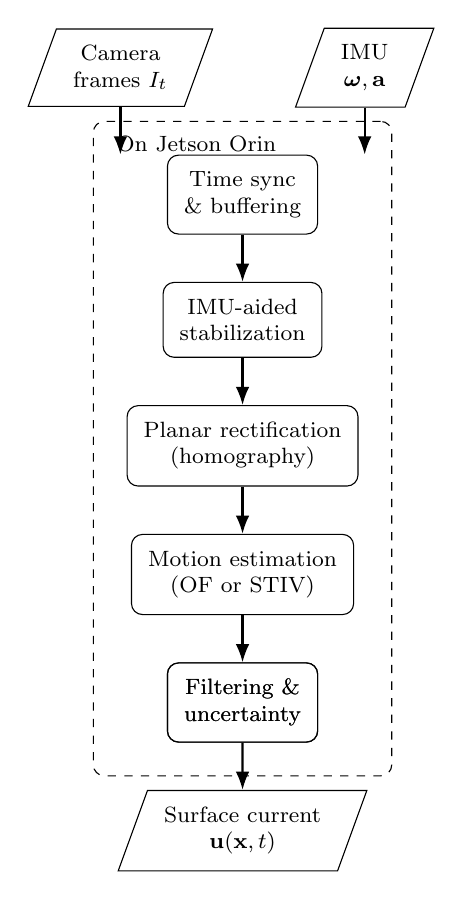
\begin{tikzpicture}[
    node distance=6mm and 4mm, % Vertical and Horizontal spacing
    font=\small,
    % Define the styles that were missing
    block/.style={
        rectangle, 
        draw, 
        rounded corners, 
        align=center, 
        minimum height=2.5em, 
        inner sep=6pt
    },
    io/.style={
        trapezium, 
        trapezium left angle=70, 
        trapezium right angle=110, 
        draw, 
        align=center, 
        inner sep=6pt
    },
    arrow/.style={
        -Latex, % Requires arrows.meta
        thick
    },
    dashedbox/.style={
        draw, 
        dashed, 
        inner sep=12pt, 
        rounded corners,
        fill=none
    }
]

% 1. Top Inputs
\node[io] (cam) {Camera\\frames $I_t$};
\node[io, right=of cam, xshift=10mm] (imu) {IMU\\$\boldsymbol{\omega},\mathbf{a}$};

% 2. Main processing chain
% We use 'calc' to center the sync block perfectly below the gap between cam and imu
\node[block, below=of $(cam.south)!0.5!(imu.south)$] (sync) {Time sync\\\& buffering};
\node[block, below=of sync] (stab) {IMU-aided\\stabilization};
\node[block, below=of stab] (rect) {Planar rectification\\(homography)};
% Note: 'motion' needs to be defined before 'post', so we insert it here
\node[block, below=of rect] (motion) {Motion estimation\\(OF or STIV)};

\node[block, below=of motion] (post) {Filtering \&\\uncertainty};



% Re-link post to ensure correct order in code if copy-pasting, 
% though TikZ solves layout non-linearly, defining order helps readability.
% (Redefined node position for clarity)
\node[block, below=of motion] (post) {Filtering \&\\uncertainty};

% 3. Output
\node[io, below=of post] (out) {Surface current\\$\mathbf{u}(\mathbf{x},t)$};

% 4. The Dashed Box (Jetson Orin)
% We fit the box around the processing nodes
\node[dashedbox, fit=(sync)(stab)(rect)(motion)(post), label={[anchor=north west, font=\footnotesize, xshift=5pt, yshift=-2pt]north west:On Jetson Orin}] (processor) {};

% 5. Connections
\draw[arrow] (cam.south) -- (sync.north -| cam.south); % Vertical-ish descent
\draw[arrow] (imu.south) -- (sync.north -| imu.south);
% Alternatively, for converging arrows matching standard flowcharts:
% \draw[arrow] (cam) -- (sync);
% \draw[arrow] (imu) -- (sync);

\draw[arrow] (sync) -- (stab);
\draw[arrow] (stab) -- (rect);
\draw[arrow] (rect) -- (motion);
\draw[arrow] (motion) -- (post);
\draw[arrow] (post) -- (out);

\end{tikzpicture}
\caption{End-to-end architecture of \textbf{OurSystem}. The IMU enables stabilization and improved rectification under platform motion.}
\label{fig:architecture}
\end{figure}

% ==========================================================
\section{Method}
\label{sec:method}
This section specifies the algorithms in a form suitable for implementation and evaluation. The undergrad implementing experiments should keep the interfaces stable and only substitute specific algorithm choices (optical flow vs STIV, different filtering models, and alternative stabilization methods).

\subsection{Calibration, Coordinate Frames, and Rectification}
Let $\mathbf{K}$ be the camera intrinsic matrix and $(\mathbf{R},\mathbf{t})$ the extrinsics mapping world coordinates to the camera frame. Assuming the water surface is a plane with unit normal $\mathbf{n}$ and signed distance $d$ from the camera center, the plane-induced homography mapping image points to an orthorectified plane can be written in standard form as
\begin{equation}
\mathbf{H} = \mathbf{K}\left(\mathbf{R} - \frac{\mathbf{t}\mathbf{n}^T}{d}\right)\mathbf{K}^{-1}.
\label{eq:homography}
\end{equation}
In practice, $\mathbf{H}$ is estimated from calibration targets, surveyed control points, or a hybrid approach consistent with operational deployments.

\begin{figure}[t]
\centering
\begin{tikzpicture}[node distance=2mm and 4mm]
\node[block] (world) {World frame\\$\{W\}$};
\node[block, right=of world] (plane) {Water plane\\$\Pi$};
\node[block, right=of plane] (camf) {Camera frame\\$\{C\}$};

\node[smallblock, below=of plane] (H) {Homography $\mathbf{H}$};
\node[io, below=of world] (img) {Image\\pixel $\mathbf{p}$};
\node[io, below=of camf] (xy) {Rectified\\$\mathbf{x}=[X,Y]^T$};

\draw[arrow] (world) -- node[above]{pose} (camf);
\draw[arrow] (plane) -- (H);
\draw[arrow] (img) -- (H);
\draw[arrow] (H) -- (xy);

\node[smallblock, below=of H, yshift=-1mm] (jac) {Flow map via Jacobian\\$\mathbf{J}_H(\mathbf{p})$};

\node[io, left=of jac, xshift=-6mm] (flowp) {Pixel flow\\$\mathbf{v}_{px}$};
\node[io, right=of jac, xshift=6mm] (flowm) {Metric flow\\$\mathbf{u}$};

\draw[arrow] (flowp) -- (jac);
\draw[arrow] (jac) -- (flowm);

\caption{Geometry and flow conversion. Rectification maps pixel locations to the water plane; a local Jacobian converts pixel/frame motion to meters/second.}
\label{fig:geometry}
\end{tikzpicture}
\end{figure}

\subsection{IMU-Aided Stabilization}
During motion, apparent image motion includes both camera motion and water motion. The IMU provides an estimate of inter-frame rotation $\widehat{\Delta \mathbf{R}}_{t\rightarrow t+\Delta t}$ from gyro integration. A practical stabilization step warps frames to a common reference orientation prior to water-plane rectification. The method implementation should expose a stable API:
\begin{equation}
(I_t', I_{t+\Delta t}') = \mathrm{Stabilize}(I_t, I_{t+\Delta t}, \widehat{\Delta \mathbf{R}}).
\end{equation}
Translational motion can be partially mitigated by plane rectification if the plane parameters are accurate; residual parallax is treated as part of the uncertainty budget.

\subsection{Motion Estimation Choices}
The pipeline supports two primary options.

Correlation-based image velocimetry estimates displacement by maximizing normalized cross-correlation between interrogation windows in rectified frames. This is closely related to LSPIV/SSIV practices.

Dense optical flow estimates a per-pixel motion field. Wavelet-based optical flow is established for nearshore foam tracking \cite{Derian2017Typhoon}, while efficient embedded models provide real-time inference paths \cite{Zhang2024NeuFlow}. The system paper should justify a specific method choice by reporting accuracy versus latency trade-offs under representative conditions.

STIV estimates streamwise (and with extensions, 2D) velocities by analyzing stripe orientation in space-time images over an accumulation window \cite{Fujita2007STIV,Han2021TwoDSTIV}. This can be compute-efficient when implemented carefully, though it trades instantaneous estimates for window-averaged outputs.

\subsection{Filtering and Uncertainty}
Outliers arise from glare, moving shadows, raindrops, camera occlusions, and regions lacking trackable texture. The post-processing stage should report both a filtered velocity field and a per-cell uncertainty estimate $\sigma_{\mathbf{u}}$, used for evaluation and for downstream sensor fusion.

\begin{algorithm}[t]
\caption{IMU-aided real-time surface current estimation (\OurSystem).}
\label{alg:pipeline}
\begin{algorithmic}[1]
\State \textbf{Input:} frames $I_t$, IMU stream $(\boldsymbol{\omega}(t),\mathbf{a}(t))$, calibration $(\mathbf{K},\mathbf{R},\mathbf{t})$, plane $\Pi$
\State \textbf{Output:} current field $\mathbf{u}(\mathbf{x},t)$, uncertainty $\sigma_{\mathbf{u}}(\mathbf{x},t)$, latency $\tau$
\State Acquire and timestamp $I_t$ and IMU samples within $[t-\epsilon, t+\Delta t+\epsilon]$
\State Estimate inter-frame rotation $\widehat{\Delta \mathbf{R}} \gets \mathrm{IntegrateGyro}(\boldsymbol{\omega})$
\State Stabilize: $(I_t', I_{t+\Delta t}') \gets \mathrm{Stabilize}(I_t, I_{t+\Delta t}, \widehat{\Delta \mathbf{R}})$
\State Rectify to water plane using $\mathbf{H}$ from \eqref{eq:homography}: $(\tilde{I}_t,\tilde{I}_{t+\Delta t}) \gets \mathrm{Rectify}(I_t', I_{t+\Delta t}', \mathbf{H})$
\State Estimate surface motion $\mathbf{v}_{px} \gets \mathrm{EstimateMotion}(\tilde{I}_t,\tilde{I}_{t+\Delta t})$
\State Convert to metric velocities $\mathbf{u} \gets \mathrm{PixelsToMeters}(\mathbf{v}_{px}, \mathbf{H}, \Delta t)$
\State Filter outliers and estimate uncertainty $(\mathbf{u},\sigma_{\mathbf{u}}) \gets \mathrm{PostProcess}(\mathbf{u}, \tilde{I}_t, \tilde{I}_{t+\Delta t})$
\State Publish $\mathbf{u}$ with timestamps and compute latency $\tau$
\end{algorithmic}
\end{algorithm}

% ==========================================================
\section{Real-Time Embedded Implementation}
\label{sec:realtime}
This section should be written as a systems contribution: it must report measured latency and throughput, and it should describe implementation decisions that materially affect performance and robustness.

A practical implementation on Jetson Orin typically uses a capture thread, an IMU thread, and a processing thread, with explicit queueing and back-pressure. The motion estimator is the primary compute cost; rectification is typically bandwidth-bound and should be GPU-accelerated when possible.

The undergrad completing this paper should implement logging of (i) per-stage runtime, (ii) queue depths, (iii) dropped frame counts, (iv) instantaneous FPS, and (v) device power and thermals. These system metrics must be measured on-device under the exact operating configuration used in accuracy experiments.

\begin{figure}[t]
\centering
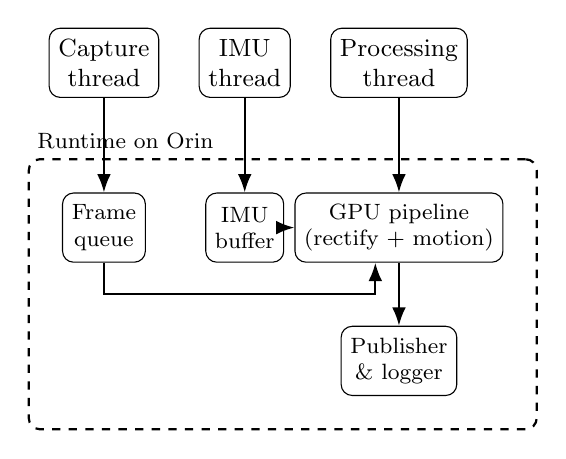
\begin{tikzpicture}[
    node distance=1.2cm and 0.5cm, % Increased vertical distance for clear separation
    block/.style={
        rectangle, 
        draw, 
        rounded corners, 
        align=center, 
        minimum height=2.5em, 
        fill=white,
        font=\small
    },
    smallblock/.style={
        rectangle, 
        draw, 
        rounded corners, 
        align=center, 
        minimum height=2.5em, 
        font=\footnotesize, 
        fill=white
    },
    dashedbox/.style={
        draw, 
        dashed, 
        inner sep=12pt, 
        rounded corners,
        thick
    },
    arrow/.style={-{Latex}, thick}
]

% Top Row: Threads
\node[block] (cap) {Capture\\thread};
\node[block, right=of cap] (imu) {IMU\\thread};
\node[block, right=of imu] (proc) {Processing\\thread};

% Bottom Row: Buffers and Pipeline
% Aligned relative to top nodes to maintain vertical flow
\node[smallblock, below=of cap] (q1) {Frame\\queue};
\node[smallblock, below=of imu] (q2) {IMU\\buffer};
\node[smallblock, below=of proc] (gpu) {GPU pipeline\\(rectify + motion)};

% Publisher below GPU
\node[smallblock, below=0.8cm of gpu] (pub) {Publisher\\\& logger};

% Vertical Arrows (Thread to Buffer/Process)
\draw[arrow] (cap) -- (q1);
\draw[arrow] (imu) -- (q2);
\draw[arrow] (proc) -- (gpu);

% Data Flow Arrows
% Route q1 to gpu underneath q2 to avoid crossing through the box
\draw[arrow] (q1.south) -- ++(0,-0.4) -| ([xshift=-0.3cm]gpu.south);
% Route q2 to gpu directly
\draw[arrow] (q2) -- (gpu);
% GPU to Publisher
\draw[arrow] (gpu) -- (pub);

% Dashed Box container
% The label is placed at the north-west anchor to sit cleanly in the gap
\node[dashedbox, fit=(q1)(q2)(gpu)(pub), label={[anchor=south west, font=\footnotesize]north west:Runtime on Orin}] (box) {};

\end{tikzpicture}
\caption{A reference concurrent design. The paper should report measured per-stage runtimes and explain back-pressure behavior under load.}
\label{fig:software}
\end{figure}

% ==========================================================
\section{Experimental Design}
\label{sec:experiments}
This section is written so an  can execute it mechanically. The core requirement is to compare \OurSystem{} against a reference measurement under controlled variation of platform motion, viewing geometry, and surface texture.

\subsection{Test Scenarios}
The experiments should include a stationary-camera baseline and a moving-platform condition. The moving-platform condition should be representative of the intended deployment, such as UAV hover jitter, mast vibration, or handheld operation from a bridge.

\subsection{Reference Measurements}
Reference options include ADCP/ADV at a nearby transect, GNSS-tracked drifters on the surface, radar surface velocity sensors, or mechanically measured point velocities in small channels where safe. The manuscript must describe synchronization between the reference and camera timestamps and must define the spatial correspondence between reference samples and image-derived estimates.

\subsection{Metrics}
Velocity error must be defined in world units, with clear averaging windows. If the output is a field, errors should be summarized both as aggregate statistics and as spatial maps of residuals. Latency must be reported as a measured distribution across time, not only as a mean value.

\begin{table}[t]
\caption{Experimental matrix template. Replace placeholder entries with the actual planned sites, conditions, and sensors.}
\label{tab:experiments}
\centering
\begin{tabular}{p{1.05cm}p{1.25cm}p{1.25cm}p{1.6cm}}
\toprule
Exp. & Platform motion & Surface texture & Reference \\
\midrule
E1 & None (tripod) & High (foam or seeded) & \TODO{e.g., drifters} \\
E2 & None (tripod) & Low (smooth/glare) & \TODO{e.g., ADCP} \\
E3 & Moderate (vibration) & High & \TODO{e.g., drifters} \\
E4 & Moderate (vibration) & Low & \TODO{e.g., ADCP} \\
E5 & UAV hover (jitter) & High & \TODO{site-dependent} \\
E6 & UAV hover (jitter) & Mixed & \TODO{site-dependent} \\
\bottomrule
\end{tabular}
\end{table}

\begin{figure}[t]
\centering
\begin{tikzpicture}[node distance=2.5mm and 4mm]
\node[block] (setup) {Set up camera+IMU\\and reference sensor};
\node[block, below=of setup] (sync) {Synchronize clocks\\and record calibration};
\node[block, below=of sync] (record) {Record video+IMU\\and reference data};
\node[block, below=of record] (run) {Run \OurSystem\\on Orin};
\node[decision, below=of run, yshift=-1mm] (qc) {Quality\\gates pass?};
\node[block, below left=of qc, xshift=-8mm] (fix) {Adjust exposure\\ROI, or filtering};
\node[block, below right=of qc, xshift=8mm] (eval) {Compute metrics\\and plots};
\node[block, below=of eval] (report) {Populate Section~\ref{sec:results}\\with results};

\draw[arrow] (setup) -- (sync);
\draw[arrow] (sync) -- (record);
\draw[arrow] (record) -- (run);
\draw[arrow] (run) -- (qc);
\draw[arrow] (qc) -- node[left]{no} (fix);
\draw[arrow] (fix) |- (run);
\draw[arrow] (qc) -- node[right]{yes} (eval);
\draw[arrow] (eval) -- (report);

\caption{Experiment execution flow. This is intended to be followed directly by the undergrad implementing and evaluating the system.}
\label{fig:expflow}
\end{tikzpicture}
\end{figure}

% ==========================================================
\section{Results}
\label{sec:results}
This section is intentionally incomplete. It should be filled by inserting measured performance and accuracy, plus ablation studies that isolate the contribution of IMU-based stabilization.

\subsection{Real-Time Performance}
\TODO{Insert a table reporting mean/median/p95 latency, sustained FPS, CPU/GPU utilization, memory bandwidth indicators if available, and power/thermals. Report values for each experiment scenario E1--E6.}

\begin{table}[t]
\caption{Real-time performance results template. Replace all TODO fields with measured values.}
\label{tab:perfresults}
\centering
\begin{tabular}{p{0.9cm}p{0.9cm}p{0.9cm}p{0.9cm}p{0.9cm}}
\toprule
Exp. & FPS & $\tau_{50}$ (ms) & $\tau_{95}$ (ms) & Power (W) \\
\midrule
E1 & \TODO{} & \TODO{} & \TODO{} & \TODO{} \\
E2 & \TODO{} & \TODO{} & \TODO{} & \TODO{} \\
E3 & \TODO{} & \TODO{} & \TODO{} & \TODO{} \\
E4 & \TODO{} & \TODO{} & \TODO{} & \TODO{} \\
E5 & \TODO{} & \TODO{} & \TODO{} & \TODO{} \\
E6 & \TODO{} & \TODO{} & \TODO{} & \TODO{} \\
\bottomrule
\end{tabular}
\end{table}

\subsection{Velocity Accuracy}
\TODO{Insert accuracy metrics compared to reference. Include spatial residual maps, scatter plots of predicted vs reference velocities, and an error-vs-range or error-vs-view-angle analysis.}

\begin{table}[t]
\caption{Accuracy results template. Replace with measured values and define the reference mapping clearly.}
\label{tab:accresults}
\centering
\begin{tabular}{p{0.9cm}p{1.2cm}p{1.2cm}p{1.2cm}}
\toprule
Exp. & MAE (m/s) & RMSE (m/s) & Bias (m/s) \\
\midrule
E1 & \TODO{} & \TODO{} & \TODO{} \\
E2 & \TODO{} & \TODO{} & \TODO{} \\
E3 & \TODO{} & \TODO{} & \TODO{} \\
E4 & \TODO{} & \TODO{} & \TODO{} \\
E5 & \TODO{} & \TODO{} & \TODO{} \\
E6 & \TODO{} & \TODO{} & \TODO{} \\
\bottomrule
\end{tabular}
\end{table}

\subsection{Ablation: Effect of IMU-Aided Stabilization}
\TODO{Provide an ablation where the same data is processed (i) with IMU stabilization and (ii) without IMU stabilization, holding all other parameters fixed. Report both accuracy and runtime impacts.}

% ==========================================================
\section{Discussion}
The discussion should interpret failure modes observed in the experiments. Common cases include weak surface texture, specular glare, rain-induced artifacts, occlusions, and significant translational motion creating parallax inconsistent with a single planar model. The paper should explain which of these are fundamental limitations and which are mitigated by improved sensing or modeling.

The discussion should also include a short privacy and deployment note. If recording in public locations, the system design should consider data minimization, on-device processing, and restricted retention of raw imagery.

% ==========================================================
\section{Conclusion}
This paper presented an IMU-aided embedded approach to real-time camera-based surface current measurement. The final version should claim only what is supported by the measured accuracy, latency, robustness, and field-validation results.

\section*{Reproducibility Artifacts}
\TODO{Provide a link to code, calibration tools, and a small anonymized dataset or a script that reproduces key figures from recorded logs. If public release is not possible, describe the artifact package structure.}

\bibliographystyle{IEEEtran}
\bibliography{refs}

\end{document}
